\documentclass[../main.tex]{subfiles}
\begin{document}

%%%%%%%%%%%%%%%%%%%%%%%%%%%%%%%
\section{\label{sect:genformal} Approaches to the sign problem: from reweighting to complex Langevin}

There have been multiple approaches suggested to solve or ameliorate the sign problem.  Some of these methods aim at solving the problem directly,
typically by rewriting the partition function in new and clever ways that remove the sign problem entirely. Other approaches involve rewriting the original problem
so it can be solved stochastically but with controlled sign fluctuations. Below we present a selection of those methods in a logical sequence that starts with
the simplest idea, namely reweighting, and concludes with complex-plane methods.
Along the way, we present an elementary discussion of each method and comment on their advantages and shortcomings, which often result in valuable insights on
the nature of the sign problem.

In \figref{SPApproaches} we propose a visual organization of the various approaches to the sign problem. Although we do not follow the proposed
taxonomy in this review in a linear fashion, we do find it helpful to organize the information in this manner. On the left column of that figure we list
``new-variables'' methods as those that attempt to tackle the sign problem by switching from the conventional path-integral formulation to a new set of
variables. We begin by reviewing a classic work that looks for sign-problem free HS transformations in \secref{AlternativeHS}.
That work shows that a choice of HS transformation may not solve the problem but may help in addressing it
(and certainly choosing the wrong one can be a recipe for trouble). Dual-variable and Majorana-fermion representations
succeed in completely solving the sign problem in many cases, as shown in Secs.~\ref{sect:DualVariables}
and~\ref{sect:Majorana}.

The middle column of \figref{SPApproaches} lists the set of what we call ``statistical" approaches, which attempt to tackle
the sign problem in a head-on manner. The simplest of those methods is by far the oldest and most commonly applied one across
all areas of physics: reweighting, which we describe in \secref{reweighting}. More recent statistical approaches,
commonly referred to as ``density-of-states'' methods, proceed by probing the shape of the probability distribution at fixed action
phase, and then integrating over that phase at the end; we describe those ideas in \secref{DensityOfStates}

Finally, the right column lists ``complex-plane" methods, which also come in different flavors. \secref{ImaginaryAsymmetry} reviews the use of imaginary asymmetries in the parameters of a given theory (e.g. chemical potential, mass imbalance) to carry out calculations without a sign problem, necessarily followed by some kind of analytic continuation to return to the real physical values.
Complex Langevin methods, the focus of this review, start in \secref{CL}, while in \secref{Thimbles} we mention ideas based on contour deformations (Lefschetz
thimbles). Both of those methods rely on complexifying the integration variables; based on that idea, there exist constructive approaches (mentioned in \secref{CL}) that aim to define a real action in such a complex space.
%
\begin{figure}[t]
  \centering
  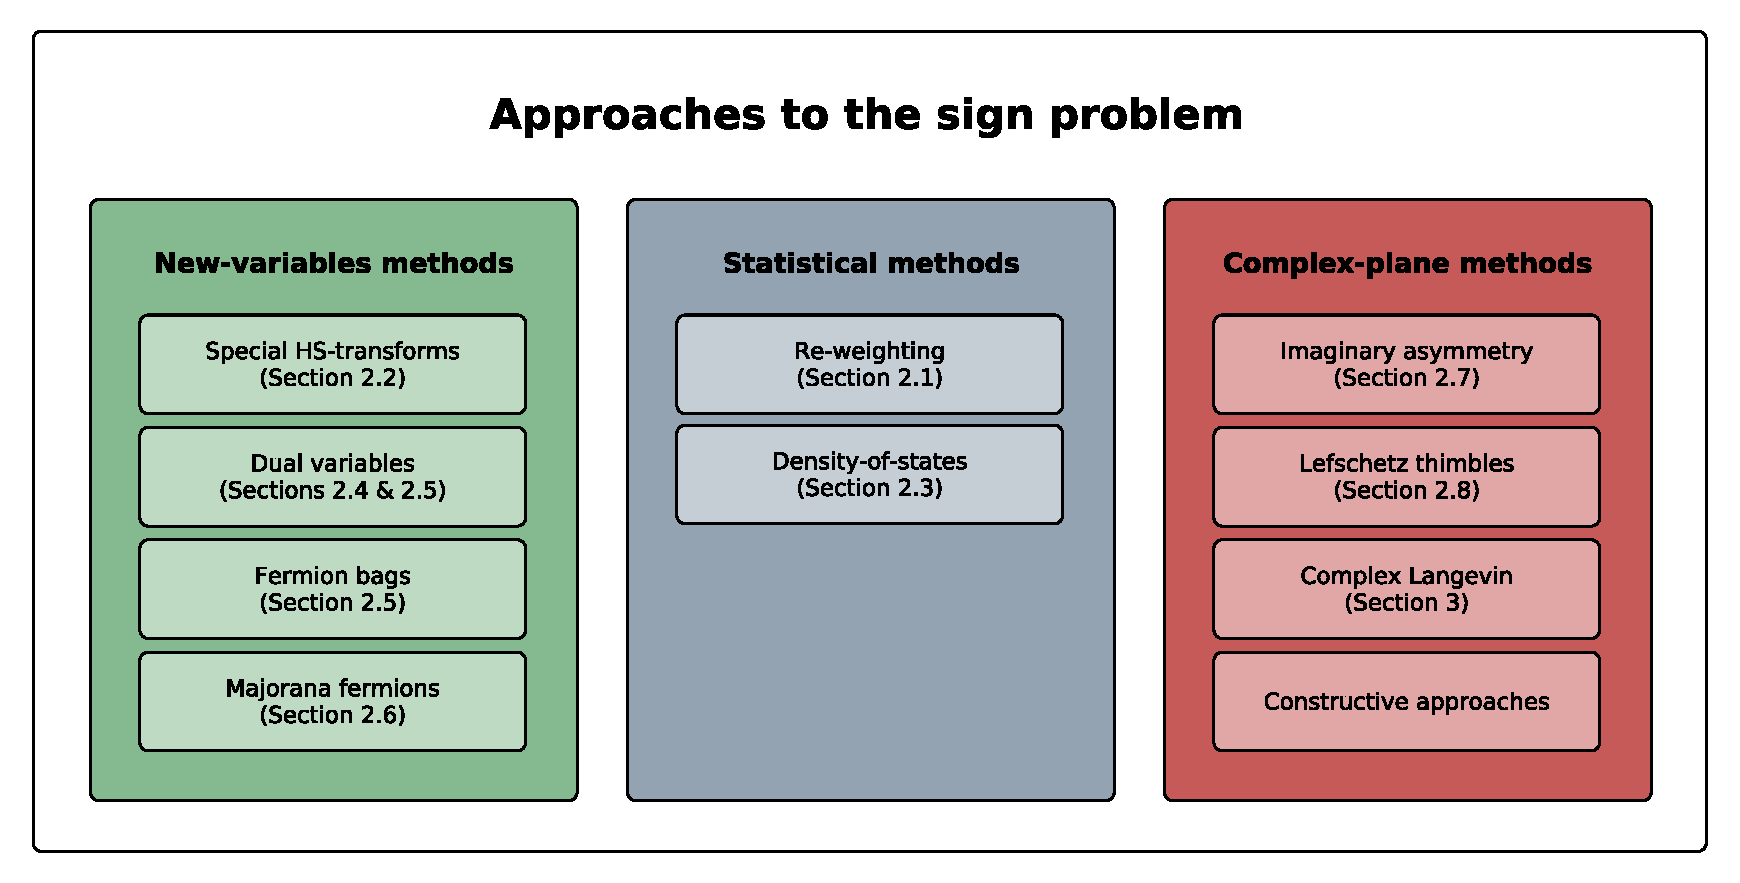
\includegraphics[width=\columnwidth]{./2generalformalism/sign_problem_solutions.pdf}
  \caption{\label{fig:SPApproaches} A proposed map of the many approaches to the sign problem.}
\end{figure}


%%%%%%%%%%%%%%%%%%%%%%%%%%%%%%%%%%
\subsection{Reweighting~\label{sect:reweighting}}

The simplest (and likely oldest~\cite{PhysRevLett.61.2635}) idea to overcome the sign problem is that of {\it reweighting}, which amounts to sampling $\phi$
using the magnitude of $P[\phi]$ as a probability measure. In such an approach, one rewrites the expectation
value of $\mathcal O$ as
%
\beq
\label{Eq:ReweightedO}
\langle  \mathcal O \rangle = \int \mathcal D \phi \; |P[\phi]| {\rm e}^{i\theta[\phi]} \mathcal O[\phi] =
\frac{\int \mathcal D \phi \; |P[\phi]| {\rm e}^{i\theta[\phi]} \mathcal O[\phi]}{\int \mathcal D \phi \; |P[\phi]|}
\frac{\int \mathcal D \phi \; |P[\phi]|}{\int \mathcal D \phi \; |P[\phi]| {\rm e}^{i\theta[\phi]}} =
\frac{\langle \langle \mathcal O [\phi] {\rm e}^{i\theta[\phi]}\rangle\rangle}{\langle\langle {\rm e}^{i\theta[\phi]}\rangle\rangle},
\eeq
%
where ${\rm e}^{i\theta[\phi]}$ is the phase of $P[\phi]$, and the double angle bracket denotes
an expectation value taken with respect to $|P[\phi]|$.

Reweighting thus provides a way forward for systems that have sign problem: simply compute the numerator and
denominator of \equref{ReweightedO}) and then take their ratio. In practice, however,
both the numerator and the denominator of \equref{ReweightedO}) vanish {\it exponentially}
as the physical extent of the spacetime lattice is increased. The phase average is
%
\beq
\langle\langle {\rm e}^{i\theta[\phi]}\rangle\rangle =
\frac{\int \mathcal D \phi \; |P[\phi]| {\rm e}^{i\theta[\phi]}}{\int \mathcal D \phi \; |P[\phi]|} = \frac{\mathcal Z}{{\mathcal Z}_{pq}} = {\rm e}^{-\beta(\Omega - \Omega_{pq})},
\eeq
%
where ${\mathcal Z}_{pq}$ is the partition function of the `phase-quenched' theory, and $\Omega_{pq}$ and $\Omega$ are the corresponding grand thermodynamic potentials of the phase-quenched and original theory. Both $\mathcal Z$ and ${{\mathcal Z}_{pq}}$ are real quantities, but since ${\mathcal Z}_{pq}$ is a sum over nonnegative real numbers, while ${\mathcal Z}$ accounts for the phase, we necessarily have ${\mathcal Z} \leq {{\mathcal Z}_{pq}}$.
More importantly, thermodynamic potentials are extensive quantities in the spatial volume $V$ of the system, such that we may write the above in terms of intensive potentials $\omega$ and $\omega_{pq}$ as
%
\beq
\label{Eq:PhaseAvg}
\langle\langle {\rm e}^{i\theta[\phi]}\rangle\rangle = {\rm e}^{-\beta V (\omega - \omega_{pq})},
\eeq
%
which exposes the exponential nature of the sign problem in the thermodynamic ($V \to \infty$) and ground-state ($\beta \to \infty$) limits.
This can be seen more clearly by examining the statistical uncertainty $\Delta$, which in a Monte Carlo calculation with ${\mathcal N}_\mathrm{s}$ samples decreases as
${\mathcal N}_\mathrm{s}^{-1/2}$.In the case of re-weighting, the relative statistical uncertainty on the average phase is overpowered by the exponential
behavior coming from \equref{PhaseAvg}:
%
\beq
\frac{\Delta}{\langle\langle {\rm e}^{i\theta[\phi]}\rangle\rangle} \sim \frac{{\rm e}^{\beta V (\omega - \omega_{pq})}}{\sqrt{\mathcal N_s}}.
\eeq
%
This last equation shows the difficulty in approaching the sign problem with a simple technique such as re-weighting: an exponentially
large number of samples is needed in order to determine the average phase with any reasonable accuracy as the volume of space time
is increased. Viewed through the lens of this simple idea, the sign problem may be regarded as the reappearance of an exponential type
of computational wall, which affects non-stochastic methods (see Introduction) in the guise of memory requirements and statistical methods
in the form of a signal-to-noise problem.

%%%%%%%%%%%%%%%%%%%%%%%%%%%%%%%%%%
\subsection{Alternative Hubbard-Stratonovich transformations\label{sect:AlternativeHS}}

The partition function $\mathcal Z$ of \equref{Z} is naturally a sum of positive quantities ${\rm e}^{-\beta(E - \mu N)}$.
The path-integral representation of $\mathcal Z$, while exact, introduces a large number of degrees of freedom to represent the
same quantity. It therefore seems natural to expect that such a formulation would {\it require} massive cancellations
(i.e. the sign problem) to yield correct physical answers. On the other hand, there are many ways to choose a HS representation,
which may in turn yield different kinds of cancellations (i.e. more or less dramatic, by some measure).
 Even in the absence of a sign problem, different kinds of continuous or discrete HS transformations display varying behavior
(see e.g.~\cite{PhysRevB.28.4059, PhysRevC.78.024001}).
It therefore makes sense to ask whether efficient representations exist, i.e. HS transformations which can substantially reduce the
difference $\omega - \omega_{pq}$ in \equref{PhaseAvg} or even eliminate it completely.

As an example, consider the fermionic Hubbard model given by
%
\beq
  \label{Eq:HubbardH}
  \hat H = -t \sum_{s=\uparrow,\downarrow}\sum_{\langle {\bf i} {\bf j}\rangle} \hat c^\dagger_{s,\bf i} \hat c^{}_{s,\bf j} + U \sum_{{\bf i}} (\hat n_{\uparrow, {\bf i}} - 1/2)(\hat n_{\downarrow, {\bf i}} - 1/2)\, ,
\eeq
%
where $t$ is the nearest-neighbor hopping, $U > 0$ is the repulsive coupling, $\hat c^{(\dagger)}_{s,\bf i}$ is the annihilation (creation) operator for particles of spin $s=\uparrow,\downarrow$ at location ${\bf i}$, and $\hat n_{s,{\bf i}}$ is the corresponding density operator.

The work of Ref.~\cite{PhysRevB.48.589} showed that a general HS transformation for the above model resulting in positive weights
(i.e. a real action $S[\phi]$) does not exist. While attractive interactions -- such as in the negative-$U$ Hubbard model -- feature no sign problem,
repulsive interactions and in general any finite polarization (i.e. non-zero chemical potential asymmetry) do yield sign oscillations.
More specifically, the problem arises because the determinant in \equref{FermionAction} becomes a product of two determinants which are
real or can be made real by choosing a proper HS transformation, but which will generally have different signs.
Reference~\cite{PhysRevB.48.589} showed that it is possible to isolate the origin of the signs in such a way that the determinants are real and
identical, i.e. one ends up with a square of a determinant, and the signs are not eliminated but can be predicted. This remarkable property is
illustrated below.

We begin by implementing a Trotter-Suzuki factorization of the Boltzmann weight with imaginary time step $\tau$, such as
%
\beq
{\rm e}^{-\tau \hat H} \simeq {\rm e}^{-\tau \hat T}  {\rm e}^{-\tau \hat V},
\eeq
%
where $\hat T$ contains the hopping terms and $\hat V$ the on-site interaction, as they appear in \equref{HubbardH}. It is to address the latter that an
HS transformation is used. The two most common HS representations, used in calculations of the repulsive Hubbard model, proceed by
writing (omitting the spatial indices)
%
\beq
\label{Eq:HSDiscrete}
{\rm e}^{-\tau U(\hat n_{\uparrow} - 1/2)(\hat n_{\downarrow} - 1/2)} = \frac{{\rm e}^{-\tau U/4}}{2} \sum_{\phi = \pm 1} {\rm e}^{-\lambda_d \phi (\hat n_{\uparrow} - \hat n_{\downarrow})},
\eeq
%
\beq
\label{Eq:HSContinuous}
{\rm e}^{-\tau U(\hat n_{\uparrow} - 1/2)(\hat n_{\downarrow} - 1/2)} = \frac{{\rm e}^{-\tau U/4}}{\sqrt{2\pi}} \int_{-\infty}^{\infty} \d\phi \; {\rm e}^{-\phi^2/2 -\lambda_c \phi (\hat n_{\uparrow} - \hat n_{\downarrow})},
\eeq
%
%
where $\phi$ is the auxiliary field, $\lambda_d$ is set by $\cosh(\lambda_d) = {\rm e}^{\tau U /2}$, and $\lambda_c = \sqrt{\tau U}$.
Both of these ``density-channel'' transformations successfully decouple the two spin species $\uparrow$ and $\downarrow$, and the
resulting determinants are real, but they are generally different from each other, such that
%
\beq
P[\phi] = \det M_\uparrow[\phi] \det M_\downarrow[\phi],
\eeq
%
will generally vary in sign with $\phi$. Here we omit the pure-$\phi$ part for the continuous case, which is real and positive anyway.
[It should be pointed out that there are more general ways than the above factorized form that result in a sign-problem free situation;
for an exploration of more general conditions based on time-reversal invariance, see Refs.~\cite{PhysRevB.71.155115, doi:10.1146/annurev-conmatphys-033117-054307}
and further discussion in \secref{Majorana}.]

A more general transformation that aims to preserve the up-down symmetry of the Hubbard Hamiltonian, and therefore provide the square of a
real determinant in $P[\phi]$, can be written as
%
\beq
{\rm e}^{-\tau U(\hat n_{\uparrow}\hat n_{\downarrow} - \hat n_{\uparrow}/2 - \hat n_{\downarrow}/2)} =
\int_{-\infty}^{\infty} \d \phi \; p[\phi] \; {\rm e}^{\phi(\hat n_{\uparrow} + \hat n_{\downarrow})},
\eeq
%
where we want $p[\phi]$ to be real and positive and, evaluating both sides at the eigenvalues of the density operators (i.e. setting $\hat n_{s} \to 0,1$), we see that
%
\bea
\int_{-\infty}^{\infty} \d \phi \; p[\phi] &=& 1, \\
\int_{-\infty}^{\infty} \d \phi \; p[\phi] {\rm e}^\phi &=& {\rm e}^{\tau U /2}, \\
\int_{-\infty}^{\infty} \d \phi \; p[\phi] ({\rm e}^\phi)^2 &=& 1.
\eea
%
Unfortunately, the last two equations can only be satisfied simultaneously if ${\rm e}^{\tau U /2} \leq 1$, i.e. if $U \leq 0$, which is not the case we are interested in here as there is then no sign problem.

The above shows that, at least within the rather general form proposed, it is not possible to generate the square of a determinant {\it and} avoid the
sign problem at the same time for the repulsive Hubbard model.
On the other hand, if $p[\phi]$ is allowed to vary in sign, then there is no constraint on $U$ and we obtain the square of a real determinant. In that
case, the sign problem comes not from the fermion determinant but from $p[\phi]$, which means that it is completely predictable as soon as $\phi$
is known, without computing determinants. Such predictability of the sign or phase of the determinant has not been exploited in the literature beyond
the work of Ref.~\cite{PhysRevB.48.589}, but it could be of interest in the context of the density-of-states methods discussed in the next section.
In those methods, the knowledge of the precise form of the imaginary part of the action as a functional of the field is essential and has been used
with some success to characterize a class of relativistic field theories.

Generally speaking, the fact that there exists a family of HS transformations representing the same partition function,
especially if they are non-trivially related to each other, provides in effect a variety of calculations that can be used as checks against each other.
As explored in Ref.~\cite{PhysRevB.42.2282},
the density-channel decompositions mentioned above can be replaced by their ``pairing channel'' counterparts
(of which a new family exists, with discrete and continuous members, as above), which display different sign properties.
Other kinds of useful HS transformations have been discussed in Refs.~\cite{PhysRevB.56.15001,doi:10.1143/JPSJ.66.1872}

Crucially, the availability of different HS transformations with different sign behavior shows that the sign problem is not an intrinsic property of
a given Hamiltonian, but rather depends on the decoupling scheme. Therefore, the search for a link between the physics of a given system and the
sign problem should be taken with caution, as such a link may be entirely an artifact of the formulation of the problem. An interesting example
in that regard is the elimination of the sign problem by way of a fermionic reformulation of a bosonic problem in the case of
a frustrated Kondo model coupled to fermions~\cite{PhysRevLett.120.107201}, followed by a HS transformation on the resulting fermionic interaction
(see also~\cite{PhysRevB.63.155114, PhysRevLett.83.796}).

It is worth pointing out, however, that there is a link between the sign problem and phase transitions. Indeed, with the path integral formulation
at hand, one can reasonably argue that the sign problem can be expected to be severe close to a critical point. One way to
visualize that concept is in terms of the Lee-Yang zeros of the partition function $\mathcal Z$, written as a path integral (i.e. \equref{PartitionZ}.
When sampled over the relevant configurations of $\phi$, the integrand ${\rm e}^{-S[\phi]}$ must reflect the existence of an accumulation point of roots of $\mathcal Z$
when approaching the phase transition. By itself, that property would not pose a problem. However, the natural scale of the integrand is
the exponential of an extensive quantity; therefore, ${\rm e}^{-S[\phi]}$ must oscillate dramatically in order to generate the large collection of zeros
(in the thermodynamic limit), and the corresponding high sensitivity to the parameter values, around the transition point. For cases that do not have
a sign problem, the integrand must necessarily tend to zero when approaching a phase transition (again, in the thermodynamic limit), which is
often reflected in the appearance of zero modes in fermion matrices.



%%%%%%%%%%%%%%%%%%%%%%%%%%%%%%%%%%
\subsection{Density-of-states methods~\label{sect:DensityOfStates}}

The density-of-states (DoS) approaches are a class of methods that attempt to tackle the sign problem in a head-on
manner, as opposed to rewriting the partition function in terms of new variables or straightforward reweighting (although it may be argued that DoS
methods are actually a kind of reweighting). The original idea of sampling the density of states as an alternative to Metropolis-based
methods is due to Wang and Landau~\cite{PhysRevLett.86.2050} and has been applied to a wide variety of systems including gauge
theories~\cite{PhysRevD.85.056010, PhysRevLett.109.111601}, but its generalization to systems with a sign problem was
explored later on in Refs.~\cite{Fodor:2007vv, PhysRevD.90.094502, 1742-6596-631-1-012063, PhysRevD.88.071502} (see also Refs.~\cite{PhysRevLett.61.2054, Schmidt:2006us}). The result of those explorations is now known
in the literature as the logarithmic linear regression (LLR) algorithm or the functional fit approach (FFA), both of which are very closely related
but differ on specific details. We will restrict ourselves here to those approaches (which have also been reviewed recently in
Ref.~\cite{Gattringer:2016kco}) but it is worth pointing out that DoS methods have also been applied to finite density QCD
in different forms which involve histograms of the phase of the fermion determinant (see e.g.~\cite{PhysRevD.77.014508, PhysRevD.78.074507, 10.1093/ptep/pts005}).

The idea common to all DoS approaches is that, in the presence of a sign problem where the action can be decomposed into real and imaginary parts
$S = S_R + iS_I$, the partition function can be written as
%
\beq
\label{Eq:ZZ}
\CZ =   \int \CD \phi \, {\rm e}^{-S[\phi]} = \int \d s \, \rho(s) \, {\rm e}^{-i s} = 2 \int \d s \, \rho(s)\, \cos(s),
\eeq
%
where we used the fact that the partition function is real and took the real part in the last step, and
%
\beq
\rho (s) = \int \CD \phi \, \delta (S_I[\phi] - s) {\rm e}^{-S_R[\phi]}.
\eeq
%
The determination of $\rho (s)$ is then carried out by combining two ingredients: first, propose a functional form that can account for its variation over vast
orders of magnitudes; second, carry out restricted calculations at constant or approximately constant imaginary action $S_I[\phi]$ in order to determine the
coefficients in the proposed functional form for $\rho (s)$. A key aspect of the method is that, using these elements, it can deliver exponential accuracy in the calculation of $\rho(s)$.

In the approach of Refs.~\cite{PhysRevD.90.094502, GATTRINGER2015545}, the parametrization of $\rho(s)$ is done in a piecewise-linear fashion:
%
\beq
\rho(s) = A_n {\rm e}^{-k_n s},
\eeq
%
for $s \in I_n$, $I_n = [s_n, s_{n+1}]$, where the partitioning and sizes of the intervals $I_n$, i.e. the set of numbers $\{ s_j \}$, can be chosen at will to
reflect the desired precision in describing $\rho(s)$. By requiring continuity of $\rho(s)$ and a normalization condition $\rho(0) = 1$, the constants $A_n$
can be determined as a function of $k_n$:
%
\beq
A_n = \exp\left(-\sum_{j=0}^{n-1} \Delta_j (k_j - k_n)\right),
\eeq
%
where $\Delta_j = s_{j+1} - s_{j}$ is the size of the $j$-th interval.
In order to determine the constants $k_n$, the FFA uses restricted expectation values defined by
%
\beq
\label{Eq:Xaverage}
\langle \langle X\rangle \rangle_n(\lambda) = \frac{\partial \ln \CZ_n(\lambda)}{\partial \lambda},
\eeq
%
where the restricted partition function is
%
\beq
\CZ_n(\lambda) = \int \CD \phi\ {\rm e}^{-S_R[\phi] + \lambda S_I[\phi]}\theta_n(S_I[\phi]),
\eeq
%
with $\theta_n(x) = 1$ for $x \in I_n$ and $0$ otherwise.

With the above piecewise-linear parametrization of $\rho(s)$, the restricted partition function and expectation values can be
computed in closed form. It turns out that
%
\beq
Y_n(\lambda) \equiv \frac{\langle \langle X\rangle \rangle_n(\lambda) - D_{n-1}}{\Delta_n} - \frac{1}{2} = h((\lambda - k_n) \Delta_n),
\eeq
%
where $D_{n-1} = \sum_{j=0}^{n-1} \Delta_j$ and
%
\beq
h(x) = \frac{1}{1 - {\rm e}^{-x}} - \frac{1}{x} - \frac{1}{2}.
\eeq
%
These equations encode a crucial aspect of the method: once the intervals $I_n$ are chosen (such that the $\Delta_n$ are fixed constants),
each of the functions $Y_n(\lambda)$ is entirely determined by the single parameter $k_n$ and must follow the shape dictated by $h(x)$.
Thus, the function $Y_n(\lambda)$ is a kind of response function in which the source parameter $\lambda$ is coupled to the imaginary
part of the action $S_I$ to constrain the value of $k_n$ for each $n$. If the one-parameter fit to $h(x)$ is unsatisfactory, that signals
a poor choice of the discretization $\{ s_j \}$, such that a more refined mesh is likely needed.
An example of the typical shape of $Y_n(\lambda)$ is shown in the left panel of \figref{FFAPlots} for several values of $n$
for the SU(3) spin model of Ref.~\cite{GIULIANI2016627}.

%
\begin{figure}[t]
  \centering
  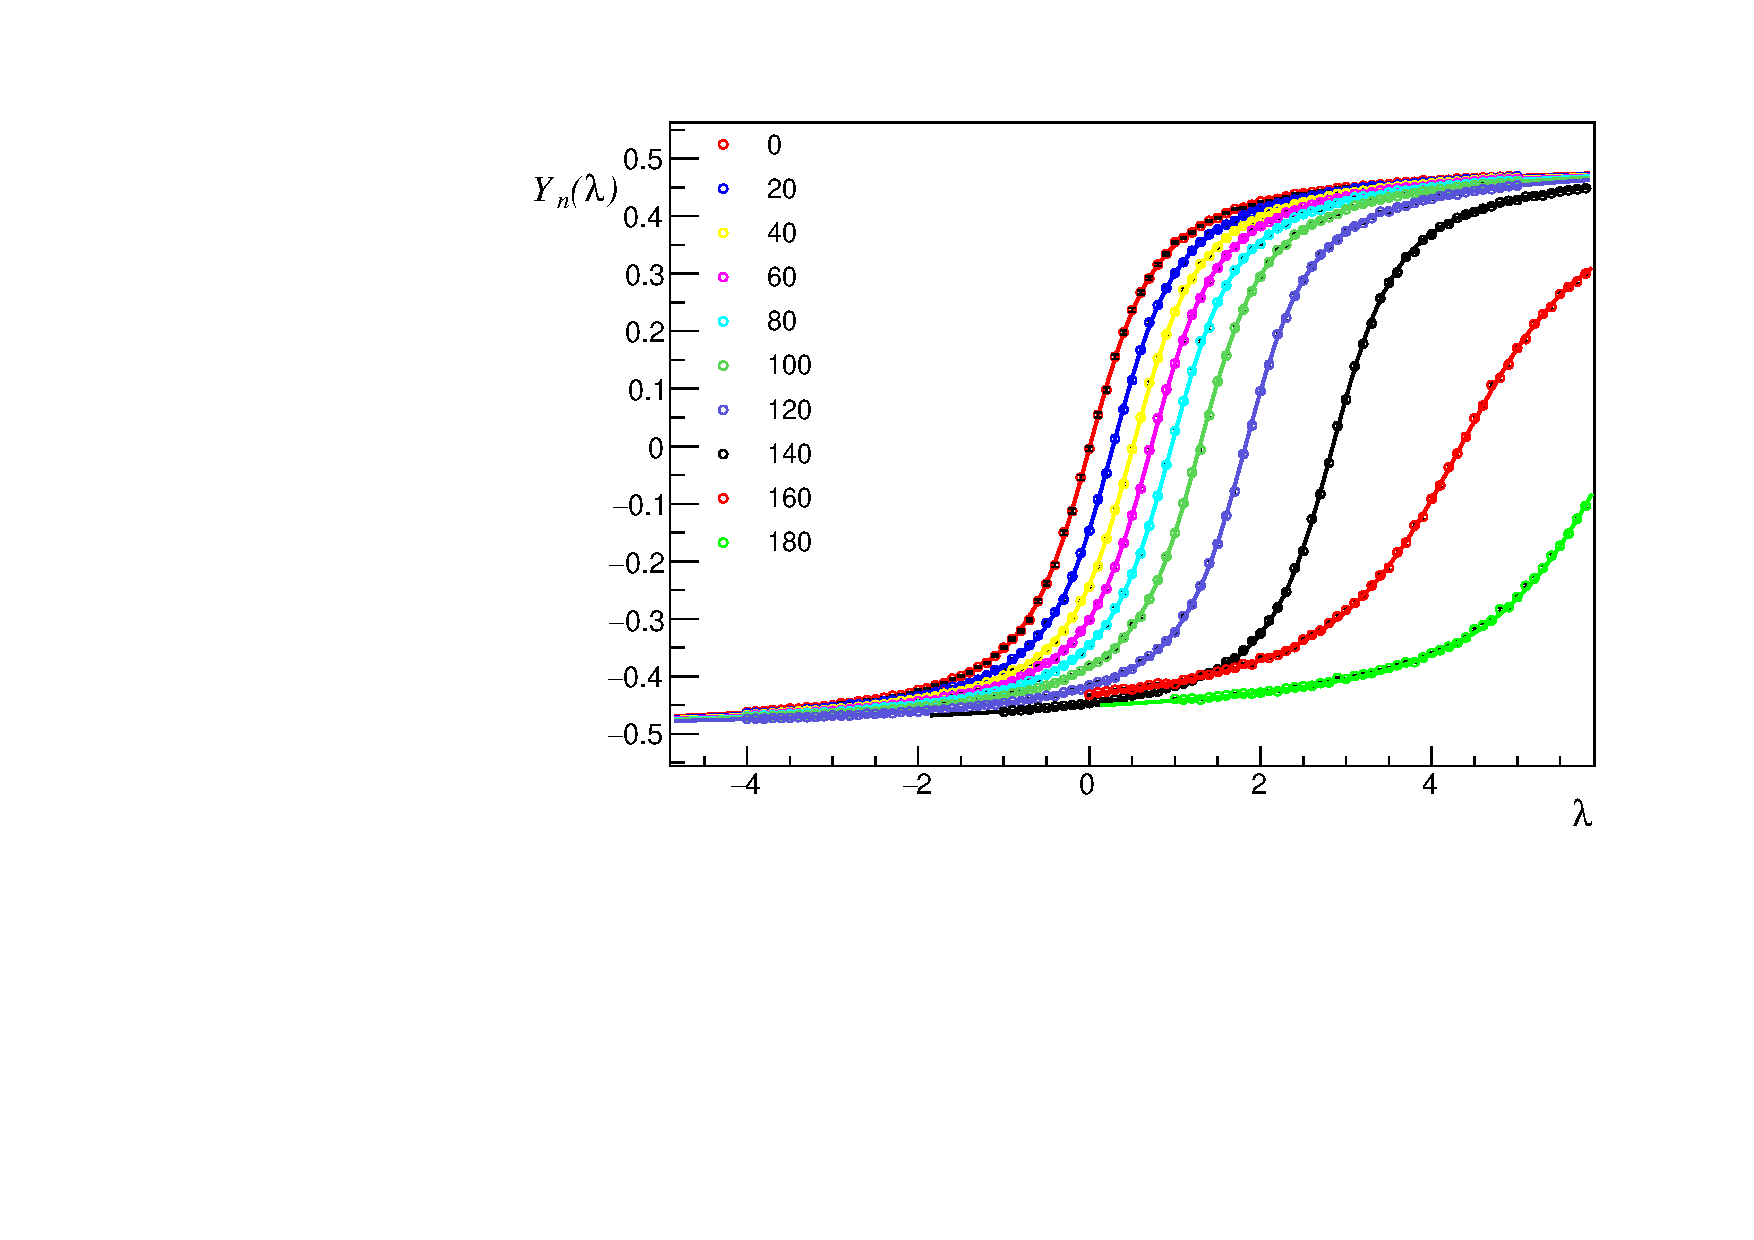
\includegraphics[width=0.53 \columnwidth]{./2generalformalism/FFAFit_example_new.pdf}
  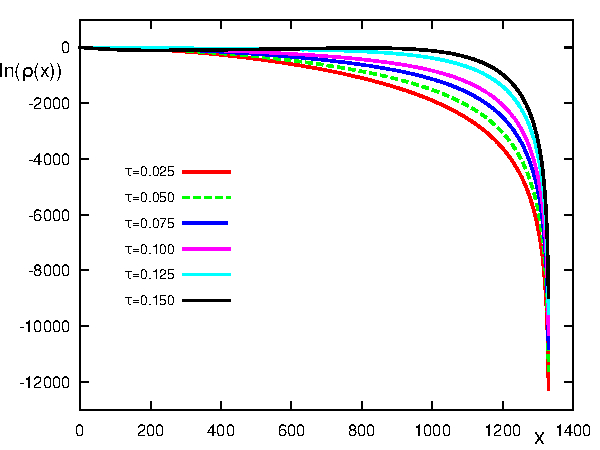
\includegraphics[width=0.46 \columnwidth]{./2generalformalism/FFArho_tau_new.pdf}
  \caption{\label{fig:FFAPlots} (Left)  $Y_n(\lambda)$ as a function of $\lambda$ for several discretizations $n$.
  (Right) Density of states for several values of the nearest-neighbor coupling $\tau$. Both plots correspond to
  the SU(3) spin model of Ref.~\cite{GIULIANI2016627}.
  }
\end{figure}
%
Once the $k_n$ are known, one may reconstruct $\rho(s)$ and calculate the full partition function as a Fourier transformation via \equref{ZZ}).
This last step will be sensitive to the large oscillations due to the $\cos(s)$ factor. As an example, the density of states obtained in Ref.~\cite{GIULIANI2016627}
for the SU(3) spin model is shown in the right panel of \figref{FFAPlots}, for several values of the nearest-neighbor coupling $\tau$. The
variations of $\rho(s)$ over many orders of magnitude are evident from that figure.

While we have focused here on the FFA, the LLR method~\cite{PhysRevLett.109.111601} accomplishes exponential error suppression by
calculating the slopes $k_n$ of the distribution using a fixed-point iteration method. The latter is based on the work of Robbins and Monro~\cite{robbins1951},
which guarantees that the values obtained in subsequent iterations are Gaussian-distributed around the exact answer.
The above-mentioned exponential error suppression amounts to a constant relative error in the determination of the density of states over the full domain
of the phase, which is crucial in order to carry out the Fourier integral in \equref{ZZ}).

The FFA and the LLR methods have been used to analyze several models on the lattice at finite
density such as the $Z_3$ spin model~\cite{GATTRINGER2015545}, the SU(3) gauge theory with static color sources~\cite{GIULIANI2016627, GIULIANI2017166},
and two-color QCD with heavy quarks~\cite{PhysRevD.88.071502}. One of the most interesting advantages of DoS methods is that they are extremely
parallelizable on modern computers. These methods require a large set of calculations, e.g. several independent calculations as a function of $\lambda$
and $n$ to determine $k_n$, but each of those is an independent run and can therefore be done in a perfectly scalable fashion. As long as the number of $\lambda$
and $n$ points does not grow exponentially with the spacetime volume (there is not indication thus far in the literature that that is the case, due largely to the
smoothness and lack of sharp features in $\ln \rho(s)$), the computational cost will scale better than that of reweighting methods.

On the other hand, DoS approaches present a paradigm that is quite different from conventional MC methods when it comes to calculating different observables.
For observables $\mathcal O$ that do not depend explicitly (and only) on the action $S[\phi]$, it will not be enough to know $\rho(s)$. In such a case,
a source term $j \mathcal O$ would have to be included in the action and a family of densities $\rho(s,j)$ would need to be calculated at least for small $j$.
Once $\rho(s,j)$ is thus obtained, numerical differentiation of $\ln \mathcal Z[j]$ yields the desired $\langle O\rangle$ in the limit $j \to 0$. Such an approach may seem
slightly cumbersome or costly, but it amounts to multiple applications of the same idea which moreover retains the full parallelizability property mentioned above.


%%%%%%%%%%%%%%%%%%%%%%%%%%%%%%%%%%
\subsection{Dual variables for bosons~\label{sect:DualVariables}}

Dualization is another approach involving rewriting the partition function $\mathcal Z$ so as to eliminate or ameliorate the sign problem.
The dual variables are a new set of variables, typically discrete, that may yield a representation of $\mathcal Z$ entirely in terms of positive quantities.
While the concept of duality is in itself an old one, the use of dual variables in quantum Monte Carlo calculations first appeared in the 1980's: for instance, Ref.~\cite{ROSSI1984105} showed that that the strong-coupling limit of QCD could be represented as a system of dimers.
Later on, Ref.~\cite{PhysRevB.61.10725} used dual variables to analyze the bosonic Hubbard model. The concept was later applied
to fermions as well, which we review in the next section. For pure bosonic theories at finite density, it was shown in Ref.~\cite{PhysRevD.75.065012} that dual
variables are not just an alternative representation: they successfully solve the sign problem for both relativistic as well as nonrelativistic systems. Moreover,
the dual variables can be efficiently sampled using the worm algorithm~\cite{PhysRevLett.87.160601, PhysRevE.66.046701}. Since the early 2010's, a few groups have pursued the
study of several quantum field theories (from simple models to effective theories of QCD) at finite temperature and density (see e.g.~\cite{PhysRevD.81.125007, PhysRevLett.106.222001, GATTRINGER2011242, Fromm:2011qi, MERCADO20121920, MERCADO2012737, Gattringer:2012df, Gattringer:2012ap}).

Following the notation and steps of Ref.~\cite{Gattringer:2016kco}, we show how to introduce dual variables first in relativistic bosons and then in the nonrelativistic case.
The lattice action for a relativistic complex valued field $\phi_x^{}$ is
%
\beq
S[\phi] = \sum_{x} \left (
\eta |\phi_x^{}|^2
+
\lambda |\phi_x^{}|^4
-
\sum_{\nu = 1}^4
\left[
{\rm e}^{\mu \delta _{\nu,4}}
\phi_x^{*}\phi_{x+\hat \nu}^{}
+
{\rm e}^{-\mu \delta _{\nu,4}}
\phi_x^{*}\phi_{x-\hat \nu}^{}
\right]
\right),
\eeq
%
where $x$ is a spacetime lattice point and $\hat \nu$ denotes a unit vector in the $\nu$-th direction ($\nu = 4$ being the imaginary-time direction).
At finite $\mu$, the quantity in square brackets ceases to be real, which exposes the sign problem. Exponentiating the action, as one would normally
do to compute the partition function, we note that
%
\beq
{\rm e}^{-S} = \prod_x {\rm e}^{-\eta |\phi_x^{}|^2 -\lambda |\phi_x^{}|^4}
\prod_{x,\nu} \exp ({\rm e}^{\mu \delta _{\nu,4}} \phi_x^{*}\phi_{x+\hat \nu}^{}) \exp ({\rm e}^{-\mu \delta _{\nu,4}} \phi_x^{}\phi_{x+\hat \nu}^{*}).
\eeq
%
At each spacetime-Lorentz point $x,\nu$, the offending term becomes a factor that can be rewritten by expanding each of the exponentials
in a Taylor series as
%
\beq
\prod_{x,\nu} \exp ({\rm e}^{\mu \delta _{\nu,4}} \phi_x^{*}\phi_{x+\hat \nu}^{}) \exp ({\rm e}^{-\mu \delta _{\nu,4}} \phi_x^{}\phi_{x+\hat \nu}^{*})
= \sum_{\{n, \bar n \}} \mathcal N_{n, \bar n} \prod_x {\rm e}^{\mu (n_{x,4} - \bar n_{x,4})}
\phi_x^{*\sum_\nu (n_{x,\nu} + \bar n_{x-\hat \nu,\nu})}
\phi_x^{\sum_\nu (\bar n_{x,\nu} + n_{x-\hat \nu,\nu})},
\eeq
%
where $\mathcal N_{n, \bar n} = \prod_{x,\nu} {1}/({n_{x,\nu}! \bar n_{x,\nu}!})$ and the sum $\sum_{\{n, \bar n \}}$ denotes a sum over all
configurations of the Taylor indices $n_{x,\nu} \geq 0$ and $\bar n_{x,\nu} \geq 0$.
Using the above and the polar form $\phi_x = r_x {\rm e}^{i\theta_x}$, we obtain for the partition function
%
\beq
\mathcal Z = \sum_{\{n, \bar n \}} \mathcal N_{n, \bar n}
\prod_x {\rm e}^{\mu (n_{x,4} - \bar n_{x,4})} R[n,\bar n,x] T[n,\bar n,x],
\eeq
%
where
%
\beq
R[n,\bar n,x] = \int_0^{\infty} \d r_x r_x^{1 + \sum_\nu \left(n_{x,\nu} + n_{x-\hat \nu,\nu} + \bar n_{x,\nu} + \bar n_{x-\hat \nu,\nu}\right)}
{\rm e}^{-\eta r_x^2 -\lambda r_x^4},
\eeq
%
which is a non-negative, local function of the index configuration $\{n, \bar n\}$ (note also that the exponent of $r_x$ is strictly positive), and
%
\beq
T[n,\bar n,x] = \int_{-\pi}^{\pi} \frac{\d \theta_x}{2\pi} {\rm e}^{-i\theta_x \sum_\nu \left(n_{x,\nu} - \bar n_{x,\nu} - n_{x-\hat \nu,\nu}  + \bar n_{x-\hat \nu,\nu}\right)},
\eeq
%
which results in Kronecker delta functions for each $x$ imposing constraints on the configurations.
In principle, the job is done at this point: we have shown that there is a discrete-field representation of the partition function as a sum
over positive quantities. It is useful, however, to take a few more steps towards simplifying the calculation, specifically towards
implementing the constraints imposed by the function $T[n,\bar n,x] $. To that end, one parameterizes the sum
and difference of $n$ and $\bar n$ via two new `dual' variables $k, \ell$ defined via
%
\beq
n_{x,\nu} - \bar n_{x,\nu} \equiv k_{x,\nu} \ \ \ \ \ \ \ \textrm{and} \ \ \ \ \ \ \ \  n_{x,\nu} + \bar n_{x,\nu} \equiv |k_{x,\nu}| + 2\ell_{x,\nu},
\eeq
%
which take values over all integers and all non-negative integers, respectively. We finally obtain
%
\beq
\mathcal Z = \sum_{k,\ell} \mathcal N_{|k| + \ell, \ell} \prod_x W(s_x) {\rm e}^{\mu \sum_x k_{x,4}} \prod_x \delta(\nabla_v k_{x,\nu}),
\eeq
%
where
%
\beq
W(n) = \int_0^{\infty} \d r r^{n+1}{\rm e}^{-\eta r^2 -\lambda r^4},
\eeq
%
\beq
s_x = \sum_\nu \left[ |k_{x,\nu}| + |k_{x-\bar\nu,\nu}| + 2(\ell_{x,\nu} + \ell_{x-\nu,\nu}) \right], \ \ \ \ \ \ \textrm{and} \ \ \ \ \ \
\nabla_v k_{x,\nu} \equiv \sum_\nu \left[k_{x,\nu} - k_{x-\hat \nu,\nu} \right].
\eeq
%
The constraint $\nabla_v k_{x,\nu} = 0$ enforces that the field $k_{x,\nu}$ be solenoidal, such that the flux of $k_{x,\nu}$ is conserved.
%Moreover, $\mu$ couples to the total flux along the time direction, which must be
%%
%\beq
%\sum_x k_{x,4} = \beta N,
%\eeq
%%
%since we know $\mu$ enters $\mathcal Z$ through the product $\mu \beta N$, where $\beta = N_\tau$ is the physical extent of the time direction, $N_\tau$ is
%the number of lattice points in that direction, and $N$ the particle number. The total flux being conserved, it must be that the temporal flux equals
%$N_\tau w[k]$, where $w[k]$ is the winding number of the flux around the time direction. Thus $N = w[k]$ and we see that the sum over
%our multiparticle Fock space has been transformed into a sum over configurations of $k,\ell$ with all possible winding numbers $w[k]$.

Pure gauge theories can also be written in terms of dual variables and, as above, results in a new representation for the partition function in
terms of purely positive terms. This approach yielded the first real and positive dualization of {\it abelian} gauge theories with a so-called $\theta$
term~\cite{PhysRevD.92.114508}, which is a term in the action coupled to a topological charge (see Refs.~\cite{Gattringer:2018dlw, Sulejmanpasic:2019ytl} for updates on that work). Because that term is necessarily complex, it results in a sign
problem in conventional path integral representations. The current challenge for this approach is the extension to {\it non-abelian} gauge theories and the
inclusion of fermions (see however next section).

The case of nonrelativistic bosons can also be addressed with dual variables with some modifications with respect to the
relativistic case. We show some of steps of that derivation here as a pedagogical example; they closely follow the relativistic case.
As we will show in more detail in \secref{NRQFT},
the problem appears in nonrelativistic bosons not because of the chemical potential but because of the asymmetry in the time derivative: there are only
particles and no antiparticles. (The physical source of the problem is thus the same as in the relativistic case: the breaking of time-reversal invariance.)
Starting with the lattice action for the complex valued field $\phi_x^{}$ in $3+1$ dimensions (although this example can be easily generalized
to $d+1$ dimensions), we have
%
\beq
S = \sum_{x} \left (
\lambda |\phi_x^{}|^4
+
\phi_x^{*}\phi_{x}^{}
-
{\rm e}^{\tau \mu}
\phi_x^{*}\phi_{x+\hat 4}^{}
-\frac{1}{2}
\sum_{k = 1}^3
\left [
\phi_x^{*}\phi_{x+\hat k}^{}
+
\phi_x^{*}\phi_{x-\hat k}^{}
-
2 \phi_x^{*}\phi_{x}^{}
\right]
\right),
\eeq
%
Then,
%
\beq
{\rm e}^{-S} = \prod_x {\rm e}^{-4 |\phi_x^{}|^2 -\lambda |\phi_x^{}|^4}
\prod_{x} \exp ({\rm e}^{\tau \mu} \phi_x^{*}\phi_{x+\hat 4}^{})
\prod_{x,k} \exp (\phi_x^{*}\phi_{x+\hat k}^{}/2) \exp (\phi_x^{*}\phi_{x-\hat k}^{}/2),
\eeq
%
where we now expand the exponentials of the derivative terms in a power series, such that
%
\bea
&& \!\!\!\!\!\!\!\!\!\!\!\!\!\!\!\!\!\!\!\!\!\!\!\!
\prod_{x} \exp ({\rm e}^{\tau \mu} \phi_x^{*}\phi_{x+\hat 4}^{})
\prod_{x,k} \exp (\phi_x^{*}\phi_{x+\hat k}^{}/2) \exp (\phi_x^{*}\phi_{x-\hat k}^{}/2) \nonumber \\
&=&
\sum_{\{n,m,\bar m\}}\;
\mathcal N_{n,m,\bar m}
{\rm e}^{\tau \mu n_x}
{\phi^*_x}^{n_x + \sum_k (m_{x,k} + \bar m_{x,k})}
{\phi^{}_x}^{n_{x-\hat 4} + \sum_k (m_{x-\hat k,k} + \bar m_{x+\hat k,k})},
\eea
%
where $\mathcal N_{n, m, \bar m} = \prod_{x} {1}/{n_{x}}! \prod_{x,k} {1}/(2^{m_{x,k}+ \bar m_{x,k}} {m_{x,k}! \bar m_{x,k}!})$,
and $n_x$ is a site variable, whereas $m_{x,k}$ and $\bar m_{x,k}$ are link variables in the spatial directions.
As in the previous example, one may now write the fields in terms of their polar representation $\phi_x = r_x {\rm e}^{i\theta_x}$ to obtain constraints for the
integer fields ${n,m,\bar m}$ and eventually arrive at a sum of positive definite terms for $\mathcal Z$. Explicitly,
%
\beq
\mathcal Z = \sum_{n,m,\bar m}\;
\mathcal N_{n,m,\bar m}
\prod_{x} {\rm e}^{\tau \mu n_x}
R[n,m,\bar m,x]
T[n,m,\bar m,x],
\eeq
%
where
%
\beq
R[n,m,\bar m,x] = \int_0^{\infty} \d r_x r_x^{1 + n_x + n_{x-\hat 4} + \sum_k \left( m_{x,k} + \bar m_{x,k} + m_{x-\hat k,k} + \bar m_{x+\hat k,k} \right)}
{\rm e}^{-4 r_x^2 -\lambda r_x^4},
\eeq
%
which is a non-negative, local function of the index configuration $\{n, m, \bar m\}$ (also, as before, the exponent of $r_x$ is strictly positive), and
%
\beq
T[n,m,\bar m,x] = \int_{-\pi}^{\pi} \frac{\d \theta_x}{2\pi} {\rm e}^{-i\theta_x \left[n_x - n_{x-\hat 4} - \sum_k \left( m_{x,k} + \bar m_{x,k} - m_{x-\hat k,k} - \bar m_{x+\hat k,k}\right)\right]},
\eeq
%
which results in Kronecker delta functions that impose constraints on the configurations.

It is then clear that the dual-variable formulation avoids the sign problem for nonrelativistic bosons, as first noted in Ref.~\cite{PhysRevD.75.065012}.
It is worth noting, however, that other cases such as coupling to angular momentum, are not obviously solvable with this technique.
%It it noteworthy that the above sum over $n$ correspond directly with the virial expansion, i.e. an expansion in powers of
%the fugacity $z = {\rm e}^{\beta \mu}$.

While this method completely solves the sign problem in the cases shown above (and some others, e.g. bosons with non-abelian spin-orbit coupling), the calculation
of specific observables acquires a new degree of complexity due to the dramatic change of variables. This is merely an algebraic
inconvenience but, in practice, the change from the original fields $\phi$ to the discrete fields $n,m,\bar{m}$ implies that any operator expression
in the $\phi$ language needs to be re-derived (e.g. by inserting sources in the original action or using the parameters of the theory).

In this section we have focused on exact alternative representations of scalar bosons. However, such representations have also been found for gauge
fields~\cite{Vairinhos:2014uxa, Vairinhos:2015ewa} which are valid also away from the strong coupling limit.

%%%%%%%%%%%%%%%%%%%%%%%%%%%%%%%%%%
\subsection{Dual variables for fermions and fermion bags}

One of the first uses of dual variables for fermions in Monte Carlo calculations was unrelated to the sign problem: it was found in
Ref.~\cite{ROSSI1984105} that QCD in the strong-coupling limit could be represented as a system of dimers, which
inspired multiple studies~\cite{WOLFF2009491, WOLFF2009549, WOLFF2010254, WOLFF2010520, PhysRevLett.104.112005,Unger:2011it}.
However, dual variables by themselves do not necessarily avoid the fermion sign problem. As first described in Ref.~\cite{PhysRevLett.83.3116},
in what is now known as the `meron cluster' approach, one must sum analytically over configurations in a given cluster (where the type of configuration
cluster must be cleverly identified) and then stochastically over clusters. When the clusters are properly chosen, they contain configurations that may vary
in sign but such that the overall contribution of a cluster is of constant sign across clusters.

The fermion bag approach of Refs.~\cite{PhysRevD.82.025007, Chandrasekharan:2013rpa} (extended to continuous time in Ref.~\cite{PhysRevD.96.114502}; see also
Refs.~\cite{Chandrasekharan2011, PhysRevLett.108.140404, PhysRevD.86.021701, PhysRevB.89.111101}) extends the meron cluster approach to a larger class of theories. Rather than following those derivations (based on Grassmann numbers), here we connect with them from a different perspective.
We begin by re-writing the partition function as
%
\beq
\mathcal Z = \textrm{Tr}\left[ {\rm e}^{-\beta (\hat H - \mu \hat N)} \right] = \textrm{Tr}\left[ \left( {\rm e}^{-\tau (\hat H - \mu \hat N)} \right)^{N_\tau} \right],
\eeq
%
where $\beta = \tau N_\tau$. Using a Suzuki-Trotter decomposition, we may approximate
%
\beq
\label{Eq:TransfMatrix}
{\rm e}^{-\tau (\hat H - \mu \hat N)} \simeq {\rm e}^{-\tau (\hat T - \mu \hat N)} {\rm e}^{-\tau \hat V},
\eeq
%
where $\hat T$ is the kinetic energy and $\hat V$ the interaction. As an example, we specialize to the case where $\hat V = -U \sum_x \hat n_\uparrow(x) \hat n_\downarrow(x)$, and then we have
%
\beq
{\rm e}^{-\tau \hat V} = \prod_x {\rm e}^{\tau U \hat n_\uparrow(x) \hat n_\downarrow(x)} = \prod_x \left( 1 + B\hat n_\uparrow(x) \hat n_\downarrow(x)\right)
=\sum_{m_{x} = 0,1} B^{\sum_{x} m_{x}} \prod_{x} \left ( \hat n_\uparrow(x) \hat n_\downarrow(x)\right)^{m_{x}}
,
\eeq
%
where  $B = {\rm e}^{\tau U} -1$. We may use the above at each point in imaginary time by inserting this
expression into \equref{TransfMatrix}) to obtain
%
\beq
{\rm e}^{-\beta (\hat H - \mu \hat N)}
= \prod_{t=1}^{N_\tau} \hat {\mathcal T}_t \prod_{x}\left( 1 + B\hat n_\uparrow(x) \hat n_\downarrow(x)\right)_t
=  \sum_{m_{x,t} = 0,1} B^{\sum_{x,t} m_{x,t}} \prod_{t=1}^{N_\tau} \left [ \hat {\mathcal T}_t \prod_{x} \left ( \hat n_\uparrow(x) \hat n_\downarrow(x)\right)^{m_{x,t}}_t \right ],
\eeq
%
where $\hat {\mathcal T}_t \equiv {\rm e}^{-\tau (\hat T - \mu \hat N)}$ and we note that the product over the time slices actually factorizes across flavors as
%
\beq
\prod_{t=1}^{N_\tau}
\left [ \hat {\mathcal T}^\uparrow_t \prod_{x} \hat n_\uparrow(x)^{m_{x,t}}_t \right ]
\prod_{t=1}^{N_\tau}
\left [ \hat {\mathcal T}^\downarrow_t \prod_{x} \hat n_\downarrow(x)^{m_{x,t}}_t \right ].
\eeq
%
Below we will show the following trace-determinant identity
%
\beq
\label{Eq:TraceDet}
\textrm{Tr} \prod_{t=1}^{N_\tau}
\left [ \hat {\mathcal T}^\uparrow_t \prod_{x} \hat n_\uparrow(x)^{m_{x,t}}_t \right ] = \det W_\uparrow[\{ m\}],
\eeq
%
where $W_s[\{ m\}]$ is the free fermion matrix for spin $s$ in which the rows and columns ${x_0,t_0}$ for which $m_{x_0,t_0} = 1$ are dropped
(see below for details on the form of $W_s[\{ m\}]$).
%
Using the above in the definition of $\mathcal Z$ yields
%
\beq
\mathcal Z = \sum_{m_{x,t} = 0,1} B^{\sum_{x,t} m_{x,t}} \det W_\uparrow[\{ m\}]\det W_\downarrow[\{ m\}],
\eeq
%
where we finally have completely re-written the full partition function as a sum over configurations of the monomer field $m_{x,t}$.

For unpolarized nonrelativistic systems, $W_s[\{ m\}]$ is real and takes on the same value for $s = \uparrow,\downarrow$, such that there is no sign problem,
as long as $B \geq 0$, i.e. for attractive interactions. Thus far, the same conditions apply for the auxiliary field formulation of the problem: repulsive interactions
($B < 0$) or polarization ($W_\uparrow[\{ m\}] \neq W_\downarrow[\{ m\}]$) would lead to a sign problem. This formulation, however, lends itself to an interpretation of the sum
in terms of clusters known as fermion bags, which are disjoint regions ${\mathcal B}_i$ of the discrete field $m_{x,t}$ within which $m_{x,t} = 0$ (see
\figref{FermionBags}). As the corresponding interaction vertices (i.e. insertions of $U$) are thus absent in $W_s[\{ m\}]$, fermions are free to move about inside the
bag. Using that property, Ref.~\cite{PhysRevD.82.025007} argued that, while the contributions to a given fermion bag configuration may vary in sign, the overall contribution
of each bag to the full partition function is actually positive. Thus, if one is able to add up the terms within each bag, then it is possible to use Metropolis-based importance
sampling to sum over all possible fermion bag configurations.

The right-hand side of \equref{TraceDet}) can also be calculated using Wick's theorem, if interpreted as the expectation value of a time-dependent operator
in a noninteracting system. In that weak-coupling interpretation, it is possible to show that
%
\beq
\label{Eq:TraceDet2}
\textrm{Tr} \prod_{t=1}^{N_\tau}
\left [ \hat {\mathcal T}^\uparrow_t \prod_{x} \hat n_\uparrow(x)^{m_{x,t}}_t \right ] = \det M_\uparrow  \det G_\uparrow[\{ m\}],
\eeq
%
where $M_\uparrow$ is the noninteracting spacetime fermion matrix and $G_\uparrow[\{ m\}]$ is a propagator matrix whose size depends on the
monomer configuration $m_{x,t}$ and which contains noninteracting propagators connecting the monomer sites where $m_{x,t} = 1$.
As explained in Ref.~\cite{Chandrasekharan:2013rpa}, the equality between Eqs.~(\ref{Eq:TraceDet}) and (\ref{Eq:TraceDet2}) represents a
duality relation between strong coupling and weak coupling; in the former case, a large number of monomers appear and \equref{TraceDet}) is easier
to calculate than \equref{TraceDet2}), which becomes easier at weak coupling.

In combination with the hopping expansion (which amounts to expanding the exponential of the
kinetic energy rather than the potential energy), one arrives at other useful sign-problem-free representations of fermionic partition functions. One such example is well-known and is the
case of nonrelativistic fermions in 1D with two-body interactions~\cite{PhysRevB.26.5033}. Another more recently discovered case is that of nonrelativistic fermions in 1D
with four-body interactions, shown and used in Refs.~\cite{PhysRevA.85.063624, PhysRevLett.109.250403, PhysRevA.87.063617}, where also a fermion-bag type idea is
used to sum over configuration clusters. Interestingly, baryons at strong coupling can also be described by bags where three quarks propagate coherently as a single free
fermion (i.e. a baryon) inside bags, while the complementary domain displays quark- and di-quark-type excitations~\cite{PhysRevD.97.074506}.
Other relevant examples can be found in Refs.~\cite{WOLFF2009549, PhysRevD.80.071503, PhysRevD.97.054501}.


\begin{figure}[t]
\floatbox[{\capbeside\thisfloatsetup{capbesideposition={right,top},capbesidewidth=0.4\textwidth}}]{figure}[\FBwidth]
{\caption{\label{fig:FermionBags} Fermion bag interpretation of the dual-variable approach to many-fermion systems. The blue dots represent the points on the
  spacetime lattice for which the discrete field acquires values $m_{x,t} = 1$. The regions enclosed by continuous black lines represent the fermion bags, within
  which $m_{x,t} = 0$ and where fermions move freely. This picture is not general but meant only as an illustration. The true shape of the allowed bag configurations will depend on the specific form of the Hamiltonian; in particular, the form of the kinetic energy operator is crucial in determining whether such a bag decomposition is possible.}}
{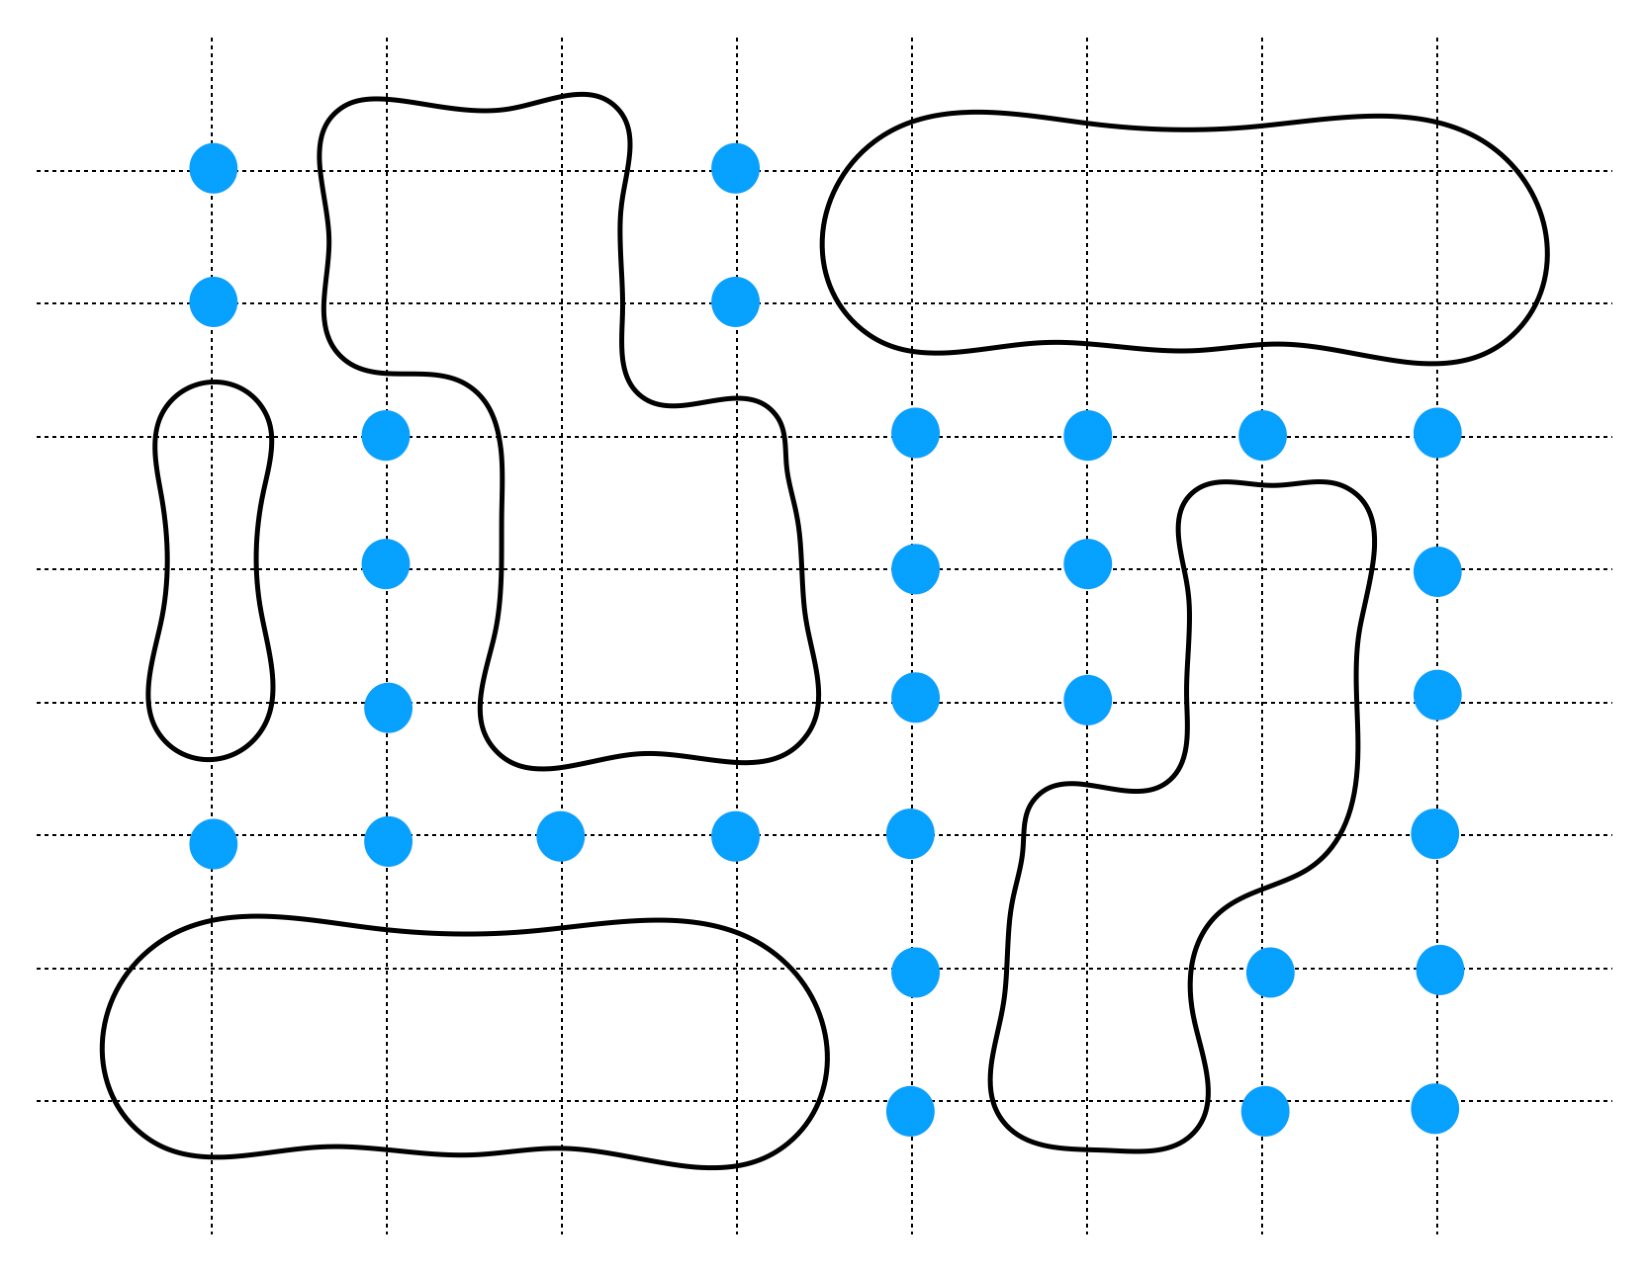
\includegraphics[width=0.55\textwidth]{./2generalformalism/FermionBags.pdf}}
\end{figure}
%
\newpage
%%%
\paragraph{Proof of trace-determinant identity}
For completeness, we outline the proof of the trace-determinant identity \equref{TraceDet}) used above.
We have not seen this way to approach the proof anywhere else, and since we find it particularly clear, we include it here.
First we quote the auxiliary identity
%
\bea
\label{Eq:AuxIDTraceDet}
\textrm{Tr}
\left[
\prod_{k=1}^{N}
{\rm e}^{\hat B_k}{\rm e}^{\hat A_k}
\right]
= \det
\left(
\begin{array}{c c c c c c}
1 & 0 &0 &0 & \cdots & {\rm e}^{B_N} \\
-{\rm e}^{A_1} & 1 &0 & 0 & \cdots & 0 \\
0 & -{\rm e}^{B_1} & 1 & \ddots & 0 & 0 \\
\vdots & \dots & \ddots & \ddots & \vdots \\
0 & 0 & -{\rm e}^{A_{N-1}} & 1  & 0\\
0 & 0 & 0 & -{\rm e}^{B_{N-1}} & 1  & 0\\
0 & 0 & 0 & \cdots & -{\rm e}^{A_{N}} & 1
\end{array}
\right ),
\eea
%
which is a reformulation of a well-known identity in the operator formulation of quantum Monte Carlo
(see e.g.~\cite{Drut:2012md}).
Here, the left-hand side trace is over Fock space, the entries of the Fermi matrix on the right-hand side are themselves matrices (i.e. the above is shown in
block form), and $\hat A_k = \sum_{i,j} [A_k]_{ij} \hat c^\dagger_i \hat c_j$ and $\hat B_k = \sum_{i,j} [B_k]_{ij} \hat c^\dagger_i \hat c_j$ are
(generally non-commuting) one-body operators.
For our purposes, $k$ represents a particular time slice, $\hat B_k = j_{x,k} \hat n_{x,k}$, such that $[{\rm e}^{B_k}]_{x,x'} = \delta_{x,x'} {\rm e}^{j_{x,k}}$, and
$\hat A_k$ encodes the kinetic energy, i.e. it is actually a $k$-independent operator. Our focus is on the $B_k$ factors.

The crucial step in proving \equref{TraceDet}) is in differentiating both sides of \equref{AuxIDTraceDet}) with respect to $j_{x,k}$ in as
many points $\{x,k\}$ as needed (namely the points where $m_{x,k} = 1$; recall each point appears only once in the matrix) to match the desired insertions of
$\hat n(x)$ at the desired time slices $k$.
To carry out the differentiations on the right-hand side, we first use the Laplace cofactor expansion of the determinant and
set the corresponding $j_{x,k}$ to zero once the derivative is taken. Once all the desired derivatives are applied, what remains is the corresponding cofactor
determinant. The latter is the determinant of the matrix on the right-hand side of \equref{AuxIDTraceDet}) where the rows and columns
of a given ${\rm e}^{B_k}$ containing the differentiated points $\{x,k\}$ are simply dropped, and the sources $j$ in any remaining terms are set to zero; that
prescription defines the square matrix $W_s[\{m\}]$, whose number of rows (and columns) is reduced from the original matrix by the number of non-zero monomers.
Note that there will, typically, be more than one spatial point $x$ affected within a given temporal block ${\rm e}^{B_k}$; similarly,
any temporal block not affected by the derivatives will turn into an identity matrix once the sources are set to zero.
Note also that any overall signs are unimportant because they cancel against the corresponding expression for the other fermion species.

%Because that appearance is in the diagonal, each derivative effectively eliminates the
%${x,k}$-th row and column and yields a constant sign times the determinant of the original Fermi matrix where row and column ${x,k}$ have been omitted.

%%%%%%%%%%%%%%%%%%%%%%%%%%%%%%%%%%
\subsection{Majorana fermions~\label{sect:Majorana}}

In Ref.~\cite{PhysRevB.91.241117} a fermion representation was introduced that does not display a sign problem for a broad class of
systems. Those developments were precipitated in part by the work of Huffman and Chadrasekharan of Ref.~\cite{PhysRevB.89.111101}.
In this representation, conventional fermionic operators $\hat \psi({\bf x})$ are written in terms of
two species of Majorana fermions $\hat \gamma_{1,2}({\bf x})$ via
%
\bea
\hat \psi({\bf x}) &=& \frac{1}{2}(\hat \gamma_{1}({\bf x}) + i \hat \gamma_{2}({\bf x}) ), \\
\hat \psi^\dagger({\bf x}) &=& \frac{1}{2}(\hat \gamma_{1}({\bf x}) - i \hat \gamma_{2}({\bf x}) ).
\eea
%
Using this representation along with a HS transformation with an auxiliary field $\phi$, it is possible to integrate out the fermionic degrees of freedom
such that the partition function then takes the form
%
\beq
\mathcal Z = \int \mathcal D \phi W_1[\phi] W_2[\phi],
\eeq
%
where
%
\beq
W_a[\phi] = +\sqrt{\det M_a[\phi]},
\eeq
%
and $M_a[\phi]$ is the Fermi matrix characterizing the dynamics of the Majorana fermions of type $a$ in the external auxiliary field $\phi$.
Under conditions of time-reversal invariance for the Majorana fermions, it is possible to show that $W_1[\phi] = W_2[\phi]^*$, such
that
%
\beq
W_1[\phi] W_2[\phi] = |W_1[\phi]|^2 \geq 0,
\eeq
%
and therefore the sign problem is completely eliminated.

A characterization of the classes of sign problems that are solved by this technique can be found in
Refs.~\cite{PhysRevLett.116.250601, PhysRevLett.117.267002} (see Ref.~\cite{Wei:2017wns} for a general and more recent
approach to such a characterization, based on semigroups).
In particular, it is worth noting that the sign problem in fully polarized (or spinless) fermions is solved by this technique.
Various applications were explored in Refs.~\cite{Li_2015, PhysRevB.92.235129, s41467-017-00167-6, PhysRevB.96.155112, PhysRevB.96.035129} and the connection with
conventional methods into a unifying principle for sign-problem free calculations, under certain symmetry conditions,
was developed in Ref.~\cite{PhysRevLett.115.250601} and Ref.~\cite{doi:10.1146/annurev-conmatphys-033117-054307}.
It should be stressed that, rather than a method or an algorithm, the Majorana representation is a way to discover systems that do not have a sign
problem (and for which it is not otherwise obvious that this is the case in conventional fermion formulations). Once that property is established, conventional algorithms can be used to carry out the calculation.

%%%%%%%%%%%%%%%%%%%%%%%%%%%%%%%%%%
\begin{figure}[t]
  \centering
  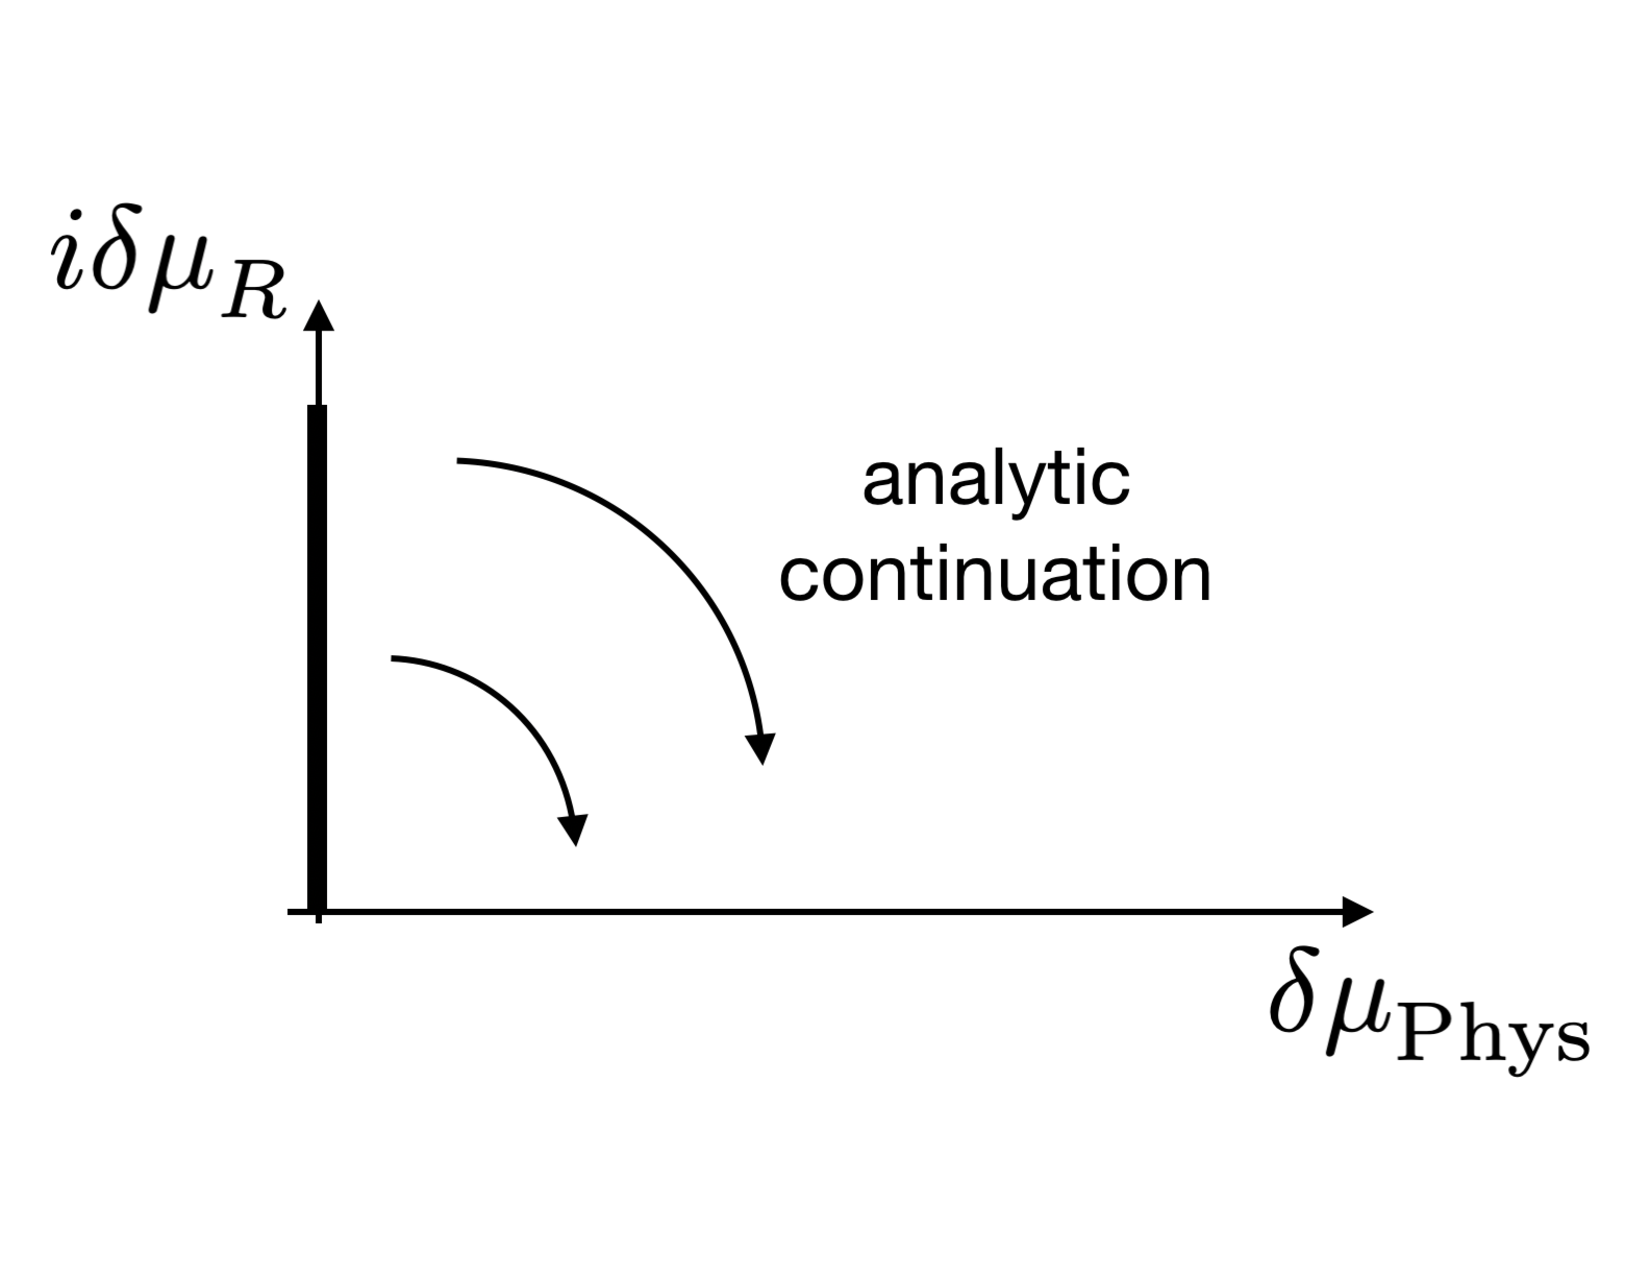
\includegraphics[width=0.49 \columnwidth]{./2generalformalism/AnalyticContinuationCartoon.pdf}
  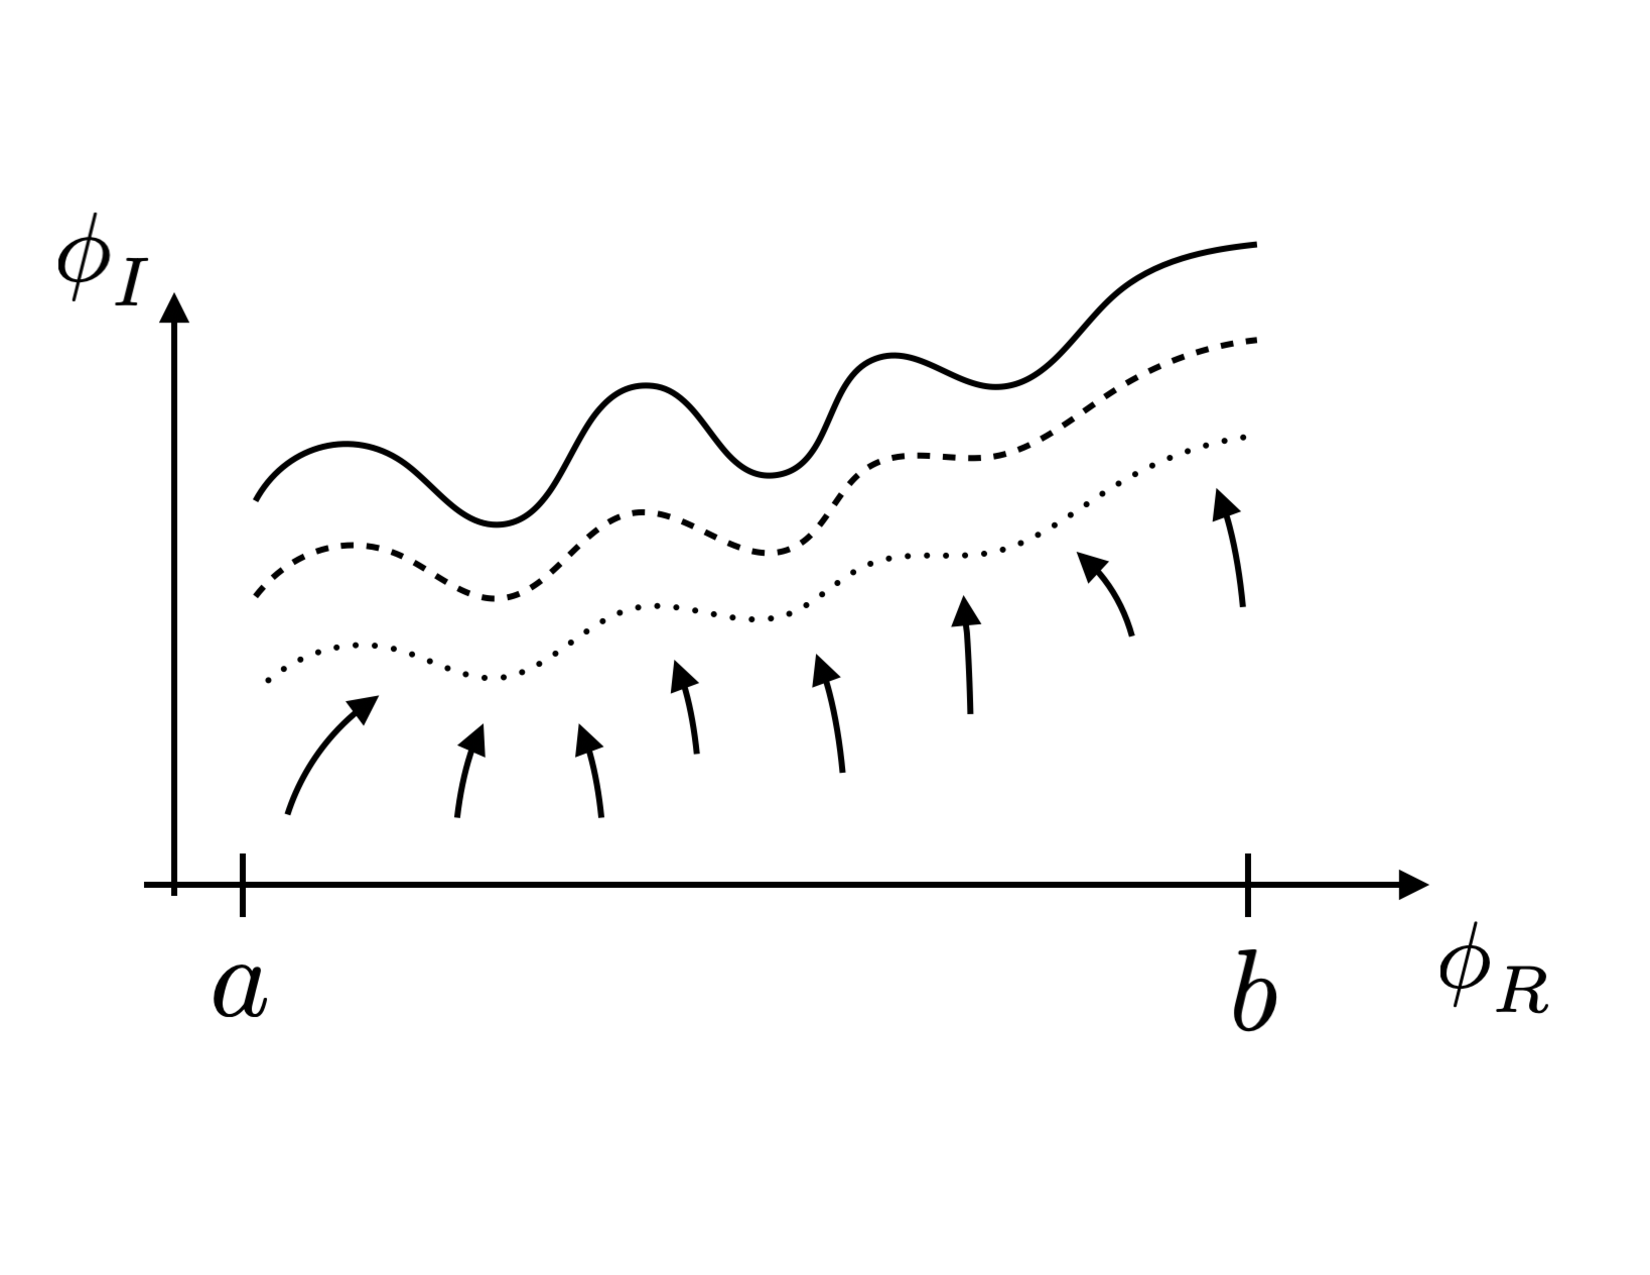
\includegraphics[width=0.49 \columnwidth]{./2generalformalism/ThimblesCartoon.pdf}
  \caption{\label{fig:ComplexPlaneMethodsCartoons} (Left) Approaches based on imaginary chemical potential asymmetry,
  as parametrized by $i \delta \mu_R$, where $\delta \mu_R$ is real, avoid the sign problem (see text) but the results must then
  be analytically continued to the physical axis where the asymmetry is real. (Right) Approaches based on deformed contour or Lefschetz thimbles
  aim to minimize the phase oscillations by numerically modifying the domain of integration of the path integral, allowing the field to acquire an imaginary part.}
\end{figure}
\subsection{Imaginary asymmetry~\label{sect:ImaginaryAsymmetry}}

Fermions at finite polarization or mass imbalance present a sign problem because although the determinant in
\equref{FermionDeterminant}) factorizes
and the factors are real, they will not typically be equal for all values of the HS field. A trick to overcome that problem,
commonly used in relativistic physics~\cite{DEFORCRAND2002290, DEFORCRAND2003170, PhysRevD.67.014505, PhysRevD.70.074509} (although its origin can be traced back to condensed matter~\cite{PhysRevB.41.811}), is to make the asymmetry imaginary.
For instance, if there are two spin flavors with
corresponding chemical potentials $\mu_{\uparrow,\downarrow} = \mu \pm \delta \mu$, then taking $\delta \mu \to i \delta \mu_R$,
where $\delta \mu_R$ is real, such that $\delta \mu$ is purely imaginary, makes the fermion determinants complex
conjugates of one another and their product is real and positive, i.e.
%
\beq
\det M_\uparrow \det M_\downarrow \to |\det M_\uparrow |^2,
\eeq
%
when ${\delta \mu \to i \delta \mu_R}$. Below, we will refer to imaginary asymmetry methods in general by the abbreviation ``iHMC''.
In relativistic physics, the equivalent of the above is the introduction of a finite chemical potential that breaks the particle-antiparticle symmetry of
the vacuum (thus inducing a finite density of particles or antiparticles, breaking time-reversal invariance and creating a sign problem).
%

%

Naturally, a caveat of this approach is that one must return to the real asymmetry axis (see left panel of \figref{ComplexPlaneMethodsCartoons}), which usually involves a fit to data and some form of analytic
continuation and thus some degree of uncontrolled approximations. The fact that investigations on the imaginary asymmetry axis are done in an
entirely nonperturbative way are certainly an attractive feature. From a practical standpoint, the idea has actually seen some important successes in
lattice QCD~\cite{PhysRevLett.105.152001, PhysRevD.85.094512, Gunther:2016vcp} (where the chemical potential must be made entirely imaginary to avoid the sign
problem; see left panel of \figref{ComplexPlaneMethodsResults}) as well as in nonrelativistic physics, where it has been applied to chemical potential as well as mass
asymmetries~\cite{Roscher:2013aqa, PhysRevLett.110.130404, PhysRevA.92.063609, PhysRevLett.114.050404, PRD96094506};
see center and right panels of \figref{ComplexPlaneMethodsResults}.
Other interesting applications, such as imaginary angular velocity, coupled to angular momentum, remain unexplored.
%


It should be pointed out that, for small asymmetries, one can avoid the problem of analytic continuation completely by performing a Taylor expansion in
the asymmetry (around vanishing asymmetry, of course). Such an approach, advocated in Ref.~\cite{deForcrand:2007rq} and used in
Ref.~\cite{Endrodi:2011gv} for QCD at finite chemical potential, can be very efficient (to the extent that the static response functions that result from the
Taylor expansion can be calculated in a statistically controlled manner). The effort on the QCD side has been pushed to sixth order in the baryon chemical potential
by the Bielefeld-BNL-CCNU collaboration, as shown in Ref.~\cite{Sharma:2017jwb}.
%%%%%%%%%%%%%%%%%%%%%%%%%%%%%%%%%%
\subsection{Lefschetz thimbles~\label{sect:Thimbles}}

In the presence of a phase problem, i.e. when the action $S[\phi]$ is complex, it may be possible to deform the contour of
integration from the real line $\phi \in (-\infty,\infty)$ into the complex plane (see right panel of \figref{ComplexPlaneMethodsCartoons})
in such a way as to make the phase of the action constant, or approximately so. Such a contour deformation changes neither the theory nor the observables,
as the integrand in the path integral of any theory of interest will be an analytic function of $\phi$.
If such a contour can be determined either a priori or dynamically during a calculation, the sign problem
could potentially be solved or at least tamed. As a Monte Carlo method, the idea can be traced back to the work of Ref.~\cite{ROM1997382} where the
so-called shifted contour auxiliary-field Monte Carlo method was put forward for electronic systems (see also Ref.~\cite{Witten:2010cx, Witten:2010zr}).
More recently, contour deformation and
Lefschetz thimbles have re-emerged as a method in quantum field
theory~\cite{PhysRevD.86.074506, PhysRevD.88.051501, PhysRevD.88.051502, Fujii:2013sra, PhysRevD.89.114505,Kanazawa2015,PhysRevD.91.101701, Fukushima:2015qza, Hayata:2015lzj, Tanizaki:2016cou, PhysRevD.95.014502, Nishimura:2017eiu, Ulybyshev:2017hbs, Bluecher:2018sgj,PhysRevD.98.034506,Ulybyshev2019fte, Ulybyshev2019hfm, Fukuma2019wbv}.

As in complex Langevin (which will be explored in the remainder of this review), the idea behind Lefschetz-thimbles approaches involves complexifying the field: $\phi \to \phi_R + i \phi_I$. One is interested in finding,
in such a complexified configuration space, the stationary points for which $\delta S/\delta \phi = 0$, as those points feature reduced phase oscillations for
$\exp\left (-i \textrm{Im} S[\phi]\right )$. Such an approach is of course the generalization of the saddle-point (or critical point) method of evaluating
complex integrals and the higher-dimensional version is often referred to as Picard-Lefschetz theory. The corresponding deformed,
high-dimensional integration contours of steepest descent are called Lefschetz thimbles.

In practice, the locations of such (stable) points of steepest descent are found by evolving the field along a fictitious time $t$ (unrelated to the imaginary time $\tau$) according to the holomorphic gradient flow equation
%
\bea
\label{Eq:HGF}
\frac{\d \phi_R}{\d t} &=& - \textrm{Re}\left[\frac{\delta S}{\delta \phi} \right],\\
\frac{\d \phi_I}{\d t} &=& + \textrm{Im}\left[\frac{\delta S}{\delta \phi} \right],\\
\eea
%
which, as we shall see below, is remarkably similar to the CL equations (see also Ref.~\cite{PhysRevD.88.094501} for a particularly
lucid side-by-side discussion of CL versus Lefschetz thimbles approaches).

The crucial advantages of deforming the path integral to capture, effectively, a set of mean-field configurations and the corresponding fluctuations,
are that $\textrm{Im} S[\phi]$ is locally constant and the real part, which determines the weight $\exp \left( - \textrm{Re} S[\phi]\right)$,
is maximally localized around the saddle point. In other words: Lefschetz thimbles are the best locations to carry out stochastic evaluations
of path integrals. While the constant-$\textrm{Im} S[\phi]$ property is crucial, the method does not rely on finding the precise location of the critical points.
Rather, it is based on finding a useful deformation which may or may not be close to the stationary phase contours attached to the critical points (wherever those
may be), but where the variations in $\textrm{Im} S[\phi]$ are small~\cite{Alexandru:2015sua}. Those ideas were crucial for the application of Refs.~\cite{PhysRevLett.117.081602, PhysRevD.95.114501} where they were used to calculate the properties of a low-dimensional field theory in real time.
Furthermore, Ref.~\cite{PhysRevD.96.034513} found that, even if the holomorphic gradient flow of \equref{HGF}) is used to push the deformation very close to the thimbles (which is
naively the ideal situation), then the high barriers separating the thimbles would make the sampling very challenging in practice.
%
\begin{figure}[t]
  \centering
  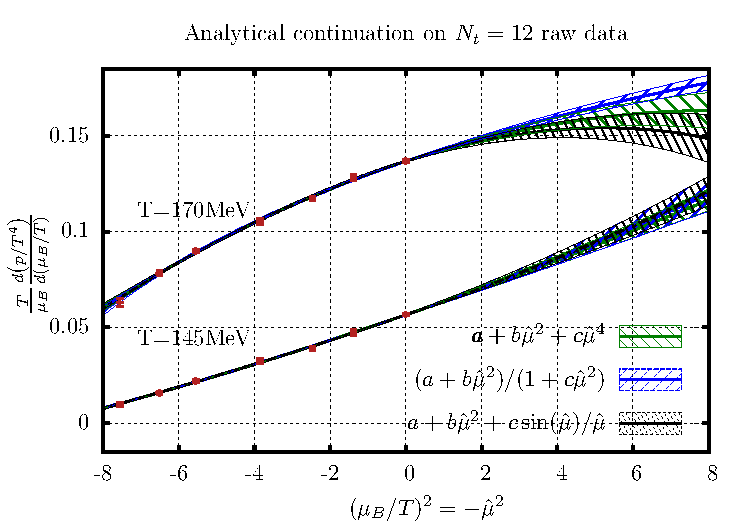
\includegraphics[width=0.45 \columnwidth]{./2generalformalism/illustrate_ana_cont.pdf}
  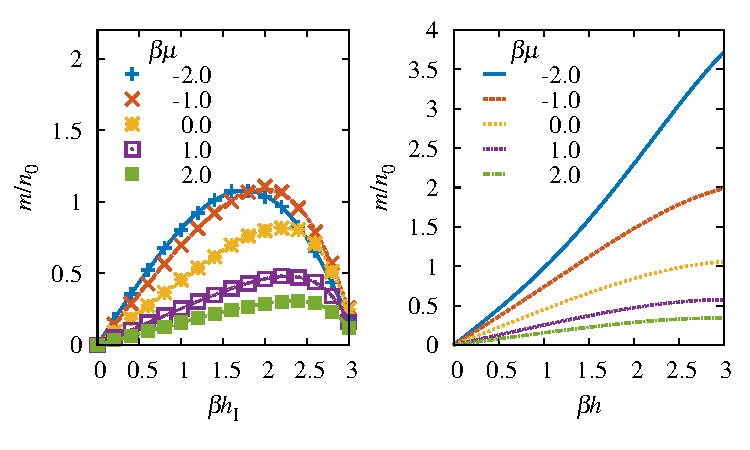
\includegraphics[width=0.52 \columnwidth]{./2generalformalism/Lambda2Magnetization.pdf}
  \caption{\label{fig:ComplexPlaneMethodsResults} (Left) Results of analytic continuation from imaginary chemical potential in QCD, from Ref.~\cite{Gunther:2016vcp}. (Middle and Right) Results for the magnetization equation of state after analytic continuation from imaginary chemical potential asymmetry $h_I$ in non-relativistic 1D fermions, from Ref.~\cite{PhysRevA.92.063609}.}
\end{figure}

One of the difficulties of deforming a contour in a functional integral is the calculation of the associated Jacobian factor~\cite{PhysRevD.93.094514}.
While that is a computational issue that is difficult but tractable, a more serious challenge lies in accounting for all the possible thimbles. The
latter is often referred to as a `global' sign problem, as opposed to the `residual' sign problem coming from the remaining curvature (i.e.
variations in the imaginary part of the Jacobian across the thimble). In that regard, it is useful to note that (for a fixed set of input parameters), only a
subset of thimbles contribute to the partition function. The global sign problem depends on the subset and the relative weights of each thimble,
both of which are difficult to determine in practice. However, the holomorphic flow bypasses that complication. It is then possible to track the global
and the residual sign problems on the deformed surface by measuring the average phase.

%%%%%%%%%%%%%%%%%%%%%%%%%%%%%%%%%%
%After this brief review of selected methods to tackle the sign problem, we arrive at the focus of this article: the CL approach. This method is a generalization of
%stochastic quantization to complex-valued variables, and allows us to treat systems with complex actions.

\end{document}
